\chapter{Oprograowanie sterownika silników}

Sterowanie silnikami zrealizowano za pomocą układu mocy VNH5019 połączonego z  STM32 Nucleo-L476RG. Oprogramowanie silników zostało stworzone w języku C oraz z wykorzystaniem bibliotek Arduino. Wiele modułów wykorzystywanych w tworzeniu robota mobilnego posiada gotowe biblioteki Arduino. Mikro kontroler jest kompatybilny z platformą Arduino Uno, pozwala to na uruchomienie programu Arduino na wykorzystywanej platformie STM32.

Do tworzenia oprogramowania użyte zostało środowisko Sloeber, które jest nakładką na zintegrowane środowisko programistyczne Eclipse. Główną zaletą Sloebera jest możliwość tworzenia oprogramowania dla platform Arduino. Środowisko rekomendowane przez producenta Arduino IDE, jest problematyczne w obsłudze w przypadku większych projektów, dlatego do tworzenia oprogramowania został wybrany Sloeber.

Stworzony program, składa się z dwóch głównych funkcji, które są standardem w przypadku programów Arduino. Pierwsza z nich \textit{setup()} odpowiada za inicjalizacje wszystkich wykorzystanych modułów. Drugą z nich jest funkcja \textit{loop()}, która jest  pętlą wykonującą się nieprzerwanie od uruchomienia programu. W niej znajduje się główny program odpowiedzialny za sterowanie i wymianę informacji z jednostką nadrzędną.

\section{Zadawanie i stabilizacja prędkości}

Sterowanie silnikami odbywa się z wykorzystaniem biblioteki od producenta jednostki mocy VNH5019 \textit{DualVNH5019MotorShield.h}. Pozwala ona na sterowanie prędkością kół poprzez zadawanie wartości sygnału PWM(ang. \textit{Pulse-Width Modulation}). 

W celu stabilizacji prędkości zastosowane zostały dwa regulatory PID, po jednym na kanał jednostki mocy.  Składa się on z trzech członów: proporcjonalnego, całkującego i różniczkującego. Ma on na celu utrzymanie prędkości obrotowej kół na zadanym poziomie. Regulator jest on opisany wzorem \ref{fig:PID_ciągły} \cite{pid_continous}.  


\begin{equation}
u(t) = K_p*e(t) + K_i*\int_{0}^{t}e(\tau )d\tau +K_d*\frac{d}{dt}e(t)
\label{fig:PID_ciągły}
\end{equation}
gdzie
\begin{eqwhere}[2cm]
	\item[$e$] uchyb regulacji 
	\item[$K_{p,i,d}$] wzmocnienia członów proporcjonalnego, całkującego i różniczkującego  
\end{eqwhere}

Uchyb regulacji to różnica między wartością zadaną oraz wartością obecną. 
Współczynnik $K_i$ i $K_d$ mogą być także zapisane jako:

\begin{equation}
K_i = K_p * T_i,   K_d = K_p * \frac{1}{T_d}
\label{fig:pid_wzmocnienia}
\end{equation}

gdzie
\begin{eqwhere}[2cm]
	\item[$T_i$] czas całkowania(zdwojenia)  
	\item[$T_d$] czas różniczkowania(wyprzedzenia)  
\end{eqwhere}

Regulator opisany równaniem \ref{fig:PID_ciągły} działa w sposób ciągły. Takie działanie jest niemożliwe do zastosowania w praktyce, ponieważ istnieje tylko skończona liczba pomiarów jakie można wykonać w danej jednostce czasu. W związku z tym zastosowany został dyskretny regulator PID opisany wzorem \ref{fig:PID_dyskretny} \cite{pid_discrete}, w którym okres próbkowania zostaje odgórnie ustalony.

\begin{equation}
u[kh] = K_p*e[kh] + K_i*\sum_{i=0}^{k}e[ih] +K_d*(e[kh]-e[kh-h])
\label{fig:PID_dyskretny}
\end{equation}
gdzie
\begin{eqwhere}[2cm]
	\item[$h$]  okres próbkowania	 
\end{eqwhere}

Okres próbkowania  został ustalony na 10ms. Wyjście z regulatora jest poddane przeskalowaniu do wartości odpowiadającej sygnałowi PWM, a następnie podane jako sterowanie na silniki.


\subsection{Wartość zadana}

Sterownik silników otrzymuje wartość zadaną  od jednostki nadrzędnej. Otrzymana wartość jest w postaci prędkości liniowej i kątowej z jaką ma poruszać się robot. Na podstawie tych prędkości została wyznaczona prędkość z jaką poruszają się prawe i lewe koła robota \cite{wheels_vel}. 

W przypadku poruszania się jednego koła, jego jeden pełen obrót powoduje przesunięcie środka wzdłuż własnej osi o dystans równy \textit{2$\pi$r}, gdzie \textit{r} jest promieniem koła. W przypadku robota posiadającego kilka obrotowych kół, każde koło obraca się wokół własnej osi i muszą one posiadać wspólny środek obrotu(Rys. \ref{fig:diff_drive2}). Ten punkt jest nazywany ICC(\textit{ang. Instantaneous Center of Curvature}). Prędkość każdego koła musi być zgodna ze sztywnym obrotem pojazdu. Oznacza to, że koła nie mogą się poruszać względem siebie.
\begin{figure}[!h]
	\centering
	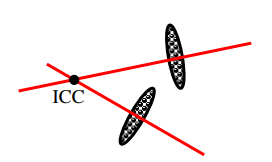
\includegraphics[scale=1]{diff_drive2.png}
	\caption{Dwa obrotowe koła muszą mieć wspólny punkt obrotu.}
	\label{fig:diff_drive2}
\end{figure}

W tworzonym robocie mobilnym koła z lewej i prawej strony poruszają się z tą samą prędkością, w związku z tym model poruszania się został uproszczony do modelu robota dwu kołowego o napędzie różnicowym(Rys. \ref{fig:diff_drive1}). 

Głównym parametrem wyprowadzenia równań kinematycznych jest prędkość kątowa $\omega$, jest zdefiniowana jako obrót każdego koła wokół punktu ICC wzdłuż koła o promieniu \textit{r}.


\begin{figure}[!h]
	\centering
	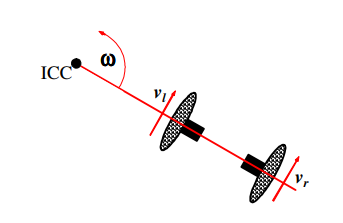
\includegraphics[scale=1]{diff_drive1.png}
	\caption{Konfiguracja kół robota z napędem różnicowym.}
	\label{fig:diff_drive1}
\end{figure}

Prędkość kół jest wyrażona wzorem \textit{v = 2$\pi$r / T} gdzie \textit{T} jest czasem pełnego obrotu wokół punktu ICC. Prędkość kątowa jest zdefiniowana jako \textit{$\omega$ = 2$\pi$ / T} i jest wyrażona w radianach na sekundę. Łącząc równania prędkości \textit{v} i \textit{$\omega$} otrzymujemy równanie \ref{fig:wr=v}.

\begin{equation}
\omega r = v
\label{fig:wr=v}
\end{equation}

Lewe i prawe koła poruszają się z różnymi prędkościami liniowymi oraz po trajektoriach posiadający różny promień, dlatego wyznaczone zostały prędkości liniowe osobne dla koła prawego(\ref{fig:wheel_r}) i lewego(\ref{fig:wheel_l}).
\begin{equation}
\omega (R+\frac{l}{2})=v_r
\label{fig:wheel_r}
\end{equation}
\begin{equation}
\omega (R-\frac{l}{2})=v_l
\label{fig:wheel_l}
\end{equation}
gdzie
\begin{eqwhere}[2cm]
	\item[$R$] odległość punktu ICC od środka robota
	\item[$l$] odległość między kołami 
\end{eqwhere}

Rozwiązując układ równań otrzymano równania opisujące prędkość kątową(\ref{fig:omega}) i promień(\ref{fig:R_rownanie}) układu. Ruch robota został zilustrowany na Rys. \ref{fig:diff_drive3}.

\begin{equation}
\omega = \frac{v_r-v_l}{l}
\label{fig:omega}
\end{equation}
\begin{equation}
R = \frac{l}{2} \frac{v_l+v_r}{v_r-v_l}
\label{fig:R_rownanie}
\end{equation}

\begin{figure}[!h]
	\centering
	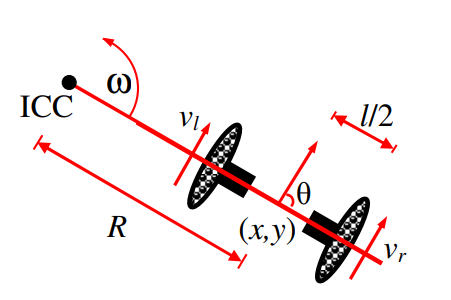
\includegraphics[scale=0.6]{diff_drive3.png}
	\caption{Ruch robota przy różnych prędkościach kół.}
	\label{fig:diff_drive3}
\end{figure}

Podstawiając \textit{$\omega$} i \textit{R} do równania \ref{fig:wr=v} otrzymano prędkość liniową z jaką porusza się robot(\ref{fig:vel_liniowa}).

\begin{equation}
v = \frac{v_l+v_r}{2}
\label{fig:vel_liniowa}
\end{equation}

Następnie wykorzystując równania \ref{fig:omega} i \ref{fig:vel_liniowa} wyznaczono prędkości liniową  prawego(\ref{fig:v_r_finish}) i lewego(\ref{fig:v_l_finish}) koła w zależności od prędkości liniowej i kątowej z jaką porusza się robot.

\begin{equation}
v_r = v + \frac{1}{2}\omega l
\label{fig:v_r_finish}
\end{equation}

\begin{equation}
v_l = v - \frac{1}{2}\omega l
\label{fig:v_l_finish}
\end{equation}

Wyznaczone prędkości liniowe lewego i prawego koła  są wartościami zadanymi regulatorów. Wyrażone są w metrach na sekundę.
\subsection{Wartość pomiarowa}

Wartością zmierzoną wykorzystywaną w regulatorach jest prędkość wyznaczona z wykorzystaniem enkoderów kwadraturowych. Liczniki impulsów zostały zrealizowane przy pomocy przerwań zewnętrznych, które wyzwalane są zboczem narastającym sygnału A(Rys. \ref{fig:encoder_quad}). W momencie wystąpienia impulsu sprawdzany jest stan sygnału B, daje to informację na temat kierunku przesunięcia fazowego sygnałów. Na tej podstawie licznik jest inkrementowany lub dekrementowany.  Enkodery po przeciwnych stronach są zliczane odwrotnie.
\begin{figure}[!h]
	\centering
	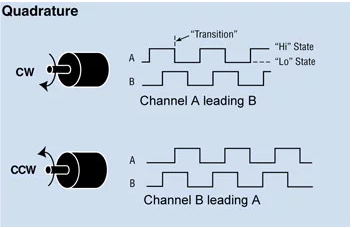
\includegraphics[scale=1]{enkodery.png}
	\caption{Przebieg sygnałów enkodera kwadraturowego \cite{encoder_quad}.}
	\label{fig:encoder_quad}
\end{figure}

Obliczenie prędkości kątowej możliwe jest dzięki wyznaczeniu zmiany kąta obrotu w czasie \cite{encoder_velocity}. Znając liczbę impulsów enkodera na pełen obrót, wyliczono o jaki kąt wykonany został obrót. Przyjęty czas próbkowania wyniósł 5ms. Wyznaczona prędkość kątowa opisana jest wzorem \ref{fig:encoder_omega}. Dysponując prędkością kątową i promieniem koła łatwo wyznaczyć prędkość liniową \ref{fig:encoder_lin}.

\begin{equation}
\omega = \frac{d\Theta}{dt} = \frac{\Delta}{T_s}=\frac{2\pi * \Delta N}{N_p * T_s}
\label{fig:encoder_omega}
\end{equation}

gdzie
\begin{eqwhere}[2cm]
	\item[$N_p$] rozdzielczość enkodera
	\item[$T_s$] czas próbkowania
	\item[$\Delta N$] ilość zliczonych impulsów  
\end{eqwhere}

\begin{equation}
v =\frac{2\pi \Delta N }{N_pT_s}R
\label{fig:encoder_lin}
\end{equation}

Wyznaczone w ten sposób prędkości liniowe poszczególnych kół pełnią role wartości pomiarowej w regulatorach. 
\section{Odometria}
\section{Jednostka inercyjna} 

Jednostka inercyjna MPU9250 posiada dedykowaną od producenta bibliotekę kompatybilną z platformą Arduino. Pozwala ona na inicjalizację komunikacji SPI lub I2C deklarując przy tym odpowiednie piny przystosowane do takich magistrali komunikacyjnych. Funkcja inicjalizacyjna zwraca informację o statusie jednostki, pozwala to na detekcje błędów przed rozpoczęciem odczytów. Biblioteka umożliwia w łatwy sposób odczyt danych z czujników. Posiada możliwość odczytu:
\begin{itemize}
	\item
	\textit{Przyspieszenia liniowego dla 3-osi }
	\item
	\textit{Prędkości liniowej dla 3-osi}
	\item 
	\textit{Orientacji w przestrzeni w postaci kwaterionu}
	\item 
	\textit{Temperatury} 
\end{itemize}